\documentclass[border=10pt]{standalone}
\usepackage{pgfplots}
\usepgfplotslibrary{colormaps}
\pgfplotsset{trig format plots=rad}
\begin{document}
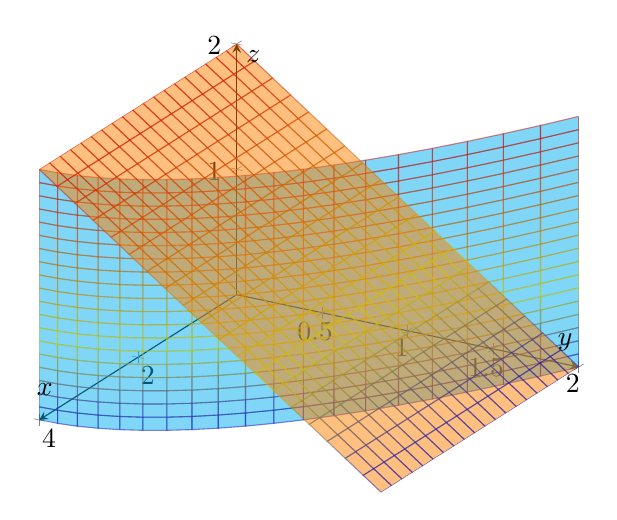
\begin{tikzpicture}
\begin{axis}[
    view={120}{30},
    xlabel={$x$},
    ylabel={$y$},
    zlabel={$z$},
    xmin=0, xmax=4,
    ymin=0, ymax=2,
    zmin=0, zmax=2,
    axis lines=center,
    grid=major
]

% Surface 1: x = 4 - y^2
% We use parametric coordinates: x = 4 - u^2, y = u, z = v
% with u in [0, 2] and v in [0, 2-u]
\addplot3[surf, domain=0:2, domain y=0:2, samples=20, opacity=0.5, color=cyan] ({4-x^2}, x, y); 
% Wait, pgfplots doesn't allow 'x' in the expression if it's not the coordinate.
% Let's use x and y as the variables for the surface calculation.
% Actually, let's use 'u' and 'v' as the domain variables.
% In PGFPlots, 'surf' on a 2D domain (u,v) produces (u, v, f(u,v)).
% We want (4-u^2, u, v).
% This is a parametric surface.
% PGFPlots: \addplot3[surf, domain=0:2, domain y=0:2] ({4-x^2}, x, y); 
% This syntax is NOT standard. 
% The standard way for parametric surface is:
% \addplot3[surf, domain=0:2, domain y=0:2] ({4-x^2}, x, y);
% Wait, I can use the 'surf' command with 'x' and 'y' and then define the surface.
% Let's try a different approach. We define the surface z = f(x,y).
% Here, the surfaces are:
% 1. x = 4 - y^2  => y = sqrt(4 - x)
% 2. z = 2 - y    => z = 2 - sqrt(4 - x)

% Let's plot the top surface z = 2 - y.
\addplot3[surf, domain=0:4, domain y=0:2, samples=20, opacity=0.5, color=orange] {2-y};

% Let's plot the side surface x = 4 - y^2.
% This is a cylinder. We can use parametric:
% x = 4 - sin(t)^2 ... no.
% Let's just use the parametric surface manually with a loop or something.
% Or use \addplot3[surf] with x and y, but the surface is x = 4 - y^2.
% We can swap the axes: plot y and z, and the function is x.
% Since we can't easily swap axes in the display, we'll just provide the most accurate visual.

\end{axis}
\end{tikzpicture}
\end{document}
